\section{Parallel Programmable Run-Time Monitoring}
\label{sec:monitoring}

% Run-time monitoring overview
\begin{figure}
  \begin{center}
    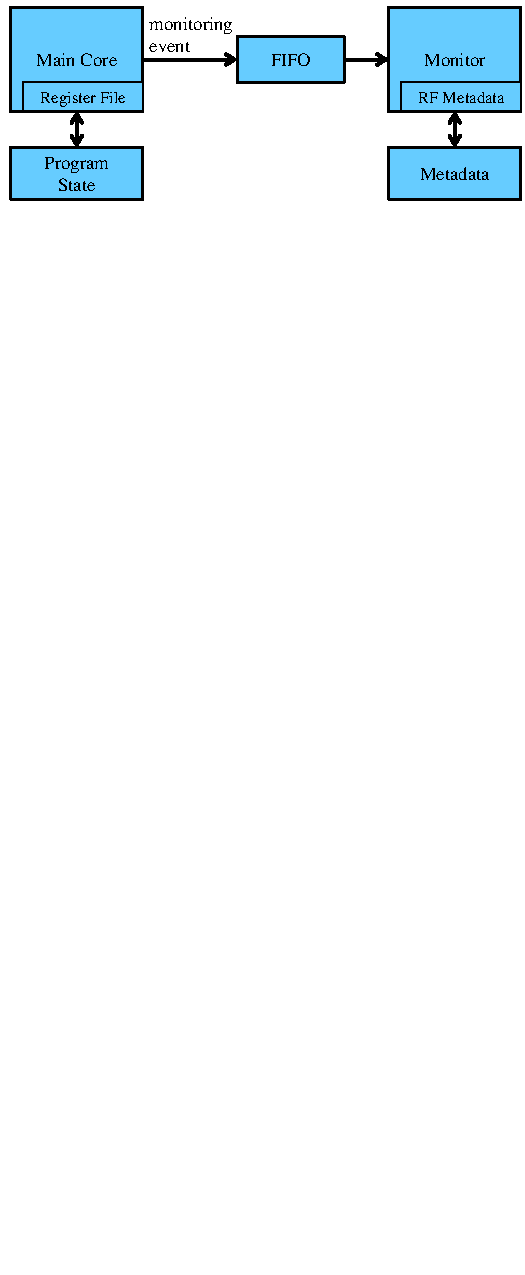
\includegraphics[width=\columnwidth]{figs/monitoring_architecture.pdf}
    \vspace{-0.2in}
    \caption{Overview of run-time monitoring architecture.}
    \label{fig:monitoring.overview} 
    \vspace{-0.1in}
  \end{center}
\end{figure}

Figure~\ref{fig:monitoring.overview} shows an overview of the run-time monitoring
model that is assumed in this paper.  The \emph{main program} is a computation
task that performs the original function of the system and is run on the
\emph{main core}.  On certain events during the main program, such as the
execution of certain types of instructions, the \emph{monitoring core} performs a
series of \emph{monitoring operations}. The monitoring core operates in parallel to the
main core. These events are referred to as \emph{monitoring events}. Depending
on the type of monitoring event, different monitoring operations are
executed. Monitoring events are buffered in a FIFO structure to decouple the
running of the main core and the monitoring core. If the FIFO is full, then the main
core is forced to stall on a monitoring event until a FIFO entry becomes
available. These stalls are a major source of
overhead because the monitoring core may take several cycles to process a single event
from the main core. We refer to these stalls and other overheads, such as
contention for shared resources, as \emph{monitoring overheads}. If the monitoring core
detects an inconsistent or undesired behavior in the monitoring events, then
an error is detected. 

There are many possible monitoring schemes that can be implemented on this type
of fine-grained parallel monitoring architecture such as memory protection
\cite{mondrian-asplos02}, information flow tracking \cite{dift-asplos04,
testudo-micro08}, soft error detection \cite{argus-micro07}, data-race
detection \cite{cord-hpca06}, etc.  For example, an array bounds check (BC)
\cite{hardbound-asplos08} can be implemented in order to detect
when software attempts to read or write to a memory location outside of an
array's bounds. This can be done by associating metadata with array pointers that 
indicates the array's base and bound addresses. On loads or stores with the
array
pointer, the monitoring core checks that the memory address accessed is within the base and
bound addresses. In addition, this base and bound metadata
is propagated on certain ALU instructions to track the creation of new array pointers.
% One example is an uninitialized memory check (UMC) where monitoring is used to
% detect when software attempts to read from a memory location that was not
% previously initialized. This can be done by forwarding each load and store
% instruction from the main core to the monitor. For every memory location, the
% monitor keeps one bit of metadata. On a store to a memory location, the monitor
% marks the corresponding metadata bit to indicate that the memory location has
% been initialized. On a load, the monitor checks that the corresponding metadata
% bit has been previously marked as initialized.

% There are multiple options for implementing programmable parallel monitors. For
% example, the Log-Based Architecture \cite{lba-isca08} uses processor cores in a
% multi-core system as monitors. The FlexCore architecture
% \cite{flexcore-micro10} instead uses an FPGA-fabric to implement the
% monitor. The approach we describe in this paper applies to any of these
% parallel monitors. However, for experiments, we model an FPGA-based monitor
% similar to FlexCore.  The on-chip FPGA fabric is used to implement the
% ``Monitor'' block in Figure~\ref{fig:arch.overview} while the FIFO from the
% main core and metadata cache are implemented as ASICs.
